\chapter{HỆ THỐNG HỖ TRỢ TUTOR CHO SINH VIÊN BÁCH KHOA}

\section{Giới thiệu}
Trong môi trường giáo dục đại học hiện nay, việc hỗ trợ học tập và phát triển kỹ năng cho
sinh viên là một nhu cầu ngày càng quan trọng. Tại Trường Đại học Bách Khoa – Đại học
Quốc gia TP.HCM (HCMUT), chương trình Tutor/Mentor đã được triển khai nhằm giúp sinh
viên được hướng dẫn, tư vấn và đồng hành trong quá trình học tập. Tuy nhiên, công tác quản
lý, phân công và theo dõi các hoạt động tutor hiện nay còn phụ thuộc nhiều vào thủ công, thiếu
tính đồng bộ và khó mở rộng. Do đó, việc phát triển một hệ thống hỗ trợ Tutor hiện đại, hiệu
quả và có khả năng tích hợp cao là rất cần thiết để đáp ứng nhu cầu quản lý và hỗ trợ học tập
trong toàn trường.

Hệ thống HCMUT\_Tutor được xây dựng nhằm hỗ trợ toàn bộ quy trình vận hành của
chương trình Tutor tại trường. Hệ thống cho phép quản lý thông tin của sinh viên và tutor
(bao gồm hồ sơ cá nhân, lĩnh vực chuyên môn, nhu cầu hỗ trợ), đồng thời cung cấp cơ chế
đăng ký, lựa chọn hoặc ghép cặp tự động giữa sinh viên và tutor. Các tutor có thể thiết lập
lịch rảnh, mở các buổi tư vấn, tổ chức buổi học trực tiếp hoặc trực tuyến, cũng như quản lý và
cập nhật thông tin buổi hướng dẫn. Hệ thống còn hỗ trợ đặt lịch, hủy lịch, đổi lịch, gửi thông
báo tự động và nhắc lịch qua giao diện hệ thống, giúp đảm bảo sự chủ động và thuận
tiện cho cả hai bên.

\section{Mô tả hệ thống}
Người dùng đăng nhập vào qua các Tài khoản (Tên đăng nhập, mật khẩu, vai trò (Student, Tutor, Staff, Admin), userID). Sinh viên và gia sư gắn với một tài khoản. Sinh viên cần lưu trữ MSSV, tên, email, department còn Gia sư thì cần Mã gia sư, tên, email, department.\\
Các sinh viên có các môn học (Subject) muốn học, còn gia sư có các môn học muốn dạy.\\
Gia sư có thể tạo các buổi học (Session) để các sinh viên tham gia, một buổi học chỉ có 1 gia sư dạy. Mỗi buổi học chỉ dạy 1 môn học, cần lưu trữ ngày bắt đầu buổi học, thời gian bắt đầu / kết thúc, kiểu buổi học (online, offline), trạng thái buổi học (Đang mở, hoàn thành), số học sinh tối đa. Nếu buổi học là online thì cần lưu trữ link meet để tham gia, còn nếu offline thì cần lưu số phòng tham gia. Trước buổi học, gia sư có thể note vào buổi học để mô tả những gì cần chuẩn bị; sau khi buổi học hoàn thành thì có thể ghi tóm tắt buổi học và link record. Gia sư có thể hoàn thành hoặc hủy buổi học để chuyển nó về trạng thái tương ứng. Gia sư có thể đổi lịch học bằng cách đổi ngày hoặc giờ bắt đầu / kết thúc.\\
Sinh viên có thể tham gia vào các buổi học nếu nó nằm trong danh sách các môn muốn học của cậu ấy và buổi học đang mở chưa đầy. Sau khi buổi học hoàn thành, sinh viên có thể đánh giá buổi học (1-5) và comment về buổi học. Sinh viên có thể gửi yêu cầu đổi lịch học (Request) đến gia sư nếu muốn đổi lịch học. Yêu cầu phải gắn với một buổi học, có ngày, giờ bắt đầu / kết thúc và lý do muốn đổi. Nếu gia sư đồng ý đổi thì buổi học sẽ đổi thành ngày giờ mới, nếu không thì không có gì xảy ra. \\
Hệ thống còn kết nối với thư viện, người dùng có thể xem các tài liệu ở đây. Các tài liệu có title, type(textbook, document, video,article), author, url. Mỗi tài liệu liên quan đến 1 hoặc nhiều môn học.\\
Hệ thống còn kết nối với một hệ thống nhắn tin để chat với nhau. Một tin nhắn có người gửi, người nhận, nội dung, thời gian, trạng thái (đã đọc / chưa đọc).\\
Hệ thống còn kết nối với một hệ thống thông báo để báo những thông tin cần thiết cho sinh viên. Một thông báo có thời gian, nội dung, loại thông báo.\\

\section{Lựa chọn DBMS}

Để xây dựng hệ thống HCMUT\_Tutor, việc lựa chọn một hệ quản trị cơ sở dữ liệu (DBMS) phù hợp là rất quan trọng. DBMS sẽ đóng vai trò trung tâm trong việc lưu trữ, quản lý và truy xuất dữ liệu của hệ thống. Sau khi phân tích các yêu cầu nghiệp vụ, nhóm đã cân nhắc giữa hai lựa chọn phổ biến là \textbf{MySQL} và \textbf{Redis}. Dưới đây là so sánh và lý do lựa chọn:

\subsection*{So sánh MySQL và Redis cho hệ thống Student-Tutor}
\begin{itemize}
    \item \textbf{MySQL} là hệ quản trị cơ sở dữ liệu quan hệ (RDBMS), hỗ trợ lưu trữ dữ liệu có cấu trúc, quan hệ phức tạp, đảm bảo tính toàn vẹn và hỗ trợ các truy vấn phức tạp (JOIN, aggregate, transaction).
    \item \textbf{Redis} là hệ quản trị cơ sở dữ liệu NoSQL dạng key-value, phù hợp cho cache, lưu trữ tạm thời, hoặc các tác vụ real-time messaging, nhưng không hỗ trợ tốt các quan hệ phức tạp, không có transaction mạnh như MySQL.
    \item Hệ thống Student-Tutor có nhiều thực thể liên kết chặt chẽ (User, Student, Tutor, Session, Subject, Review, Request), cần đảm bảo tính toàn vẹn dữ liệu, hỗ trợ truy vấn tổng hợp, thống kê, và các thao tác đồng thời (ví dụ: đăng ký buổi học, đánh giá, đổi lịch).
    \item Redis có thể dùng bổ sung cho các chức năng như cache, queue thông báo, hoặc chat real-time, nhưng không phù hợp làm DBMS chính cho hệ thống nghiệp vụ phức tạp.
\end{itemize}

\subsection*{Lý do chọn MySQL làm DBMS chính}
\begin{itemize}
    \item \textbf{Dữ liệu quan hệ phức tạp:} Hệ thống có nhiều bảng liên kết (nhiều-nhiều, một-nhiều), cần JOIN và ràng buộc toàn vẹn dữ liệu.
    \item \textbf{Hỗ trợ transaction mạnh:} Đảm bảo các thao tác như đăng ký buổi học, đổi lịch, đánh giá đều nhất quán, tránh double-booking hoặc mất dữ liệu.
    \item \textbf{Truy vấn tổng hợp và thống kê:} MySQL hỗ trợ tốt các phép tính tổng hợp (COUNT, AVG, SUM, GROUP BY) phục vụ dashboard, báo cáo.
    \item \textbf{Khả năng mở rộng và hiệu suất:} MySQL có thể mở rộng theo chiều ngang (replication, clustering), đáp ứng nhu cầu tăng trưởng người dùng.
    \item \textbf{Bảo mật và sao lưu:} MySQL hỗ trợ nhiều cơ chế bảo mật, backup/restore dữ liệu hiệu quả.
    \item \textbf{Tích hợp tốt với Python/Flask:} Dễ dàng phát triển backend, ORM (SQLAlchemy), triển khai trên nhiều nền tảng.
    \item \textbf{Cộng đồng lớn, chi phí thấp:} Tài liệu phong phú, dễ tìm giải pháp, tiết kiệm chi phí triển khai.
\end{itemize}

\textbf{Kết luận:} \textit{MySQL là lựa chọn tối ưu cho hệ thống Student-Tutor do đáp ứng tốt các yêu cầu về dữ liệu quan hệ, tính toàn vẹn, hiệu suất, bảo mật và khả năng mở rộng. Redis chỉ nên dùng bổ trợ cho cache hoặc các chức năng real-time, không phù hợp làm DBMS chính.}

\section{ERD and Mapping}
\begin{figure}[H]
    \centering
    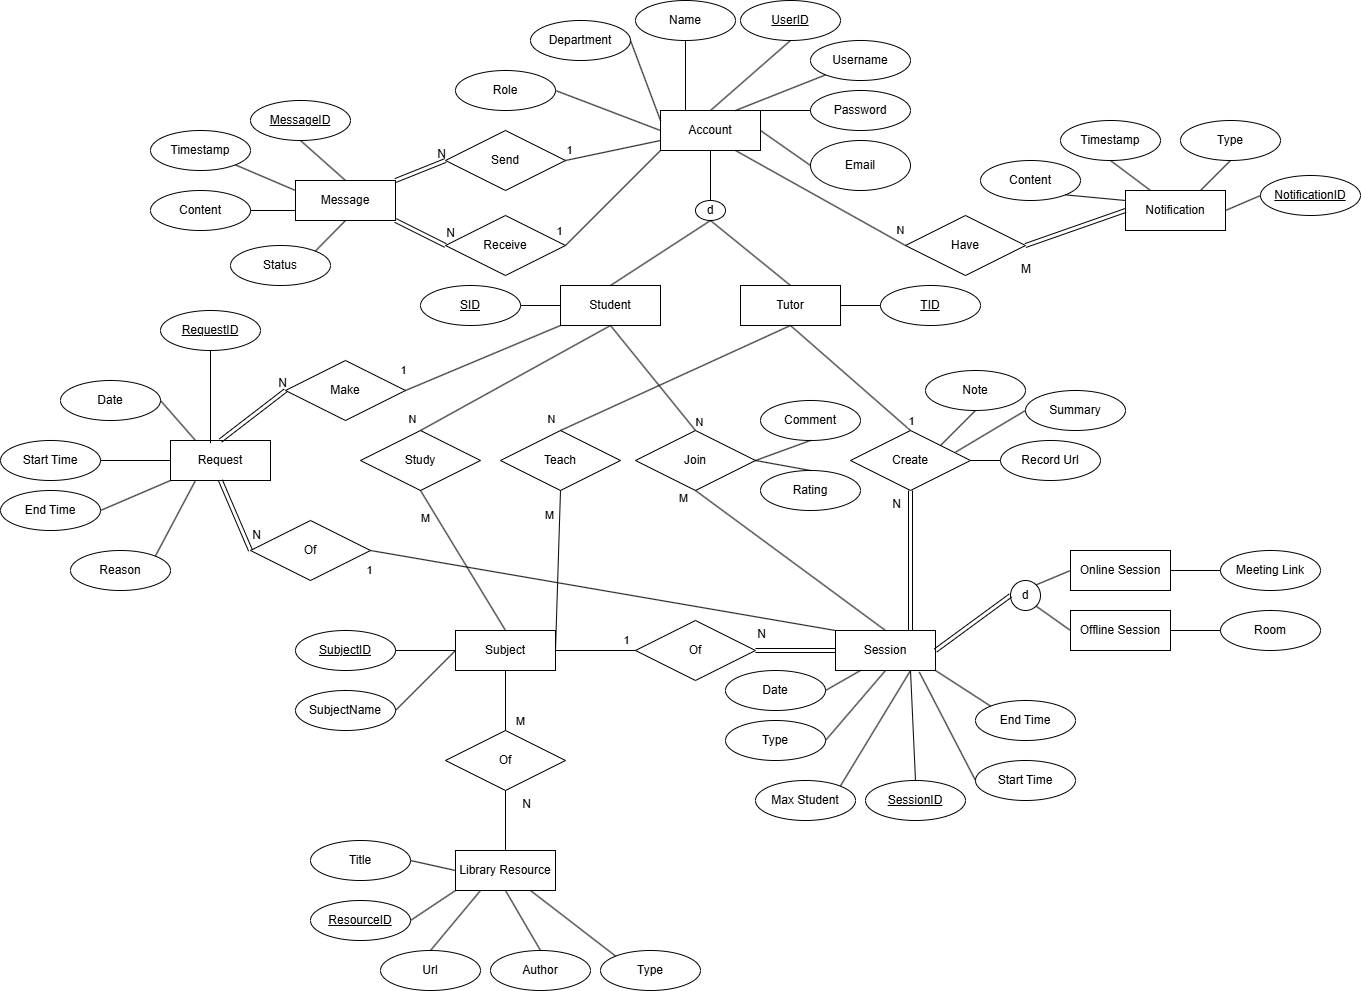
\includegraphics[width=0.8\textwidth]{figures/Kha/erd.drawio.png}
    \caption{ERD của hệ thống HCMUT\_Tutor}
\end{figure}

\begin{figure}[H]
    \centering
    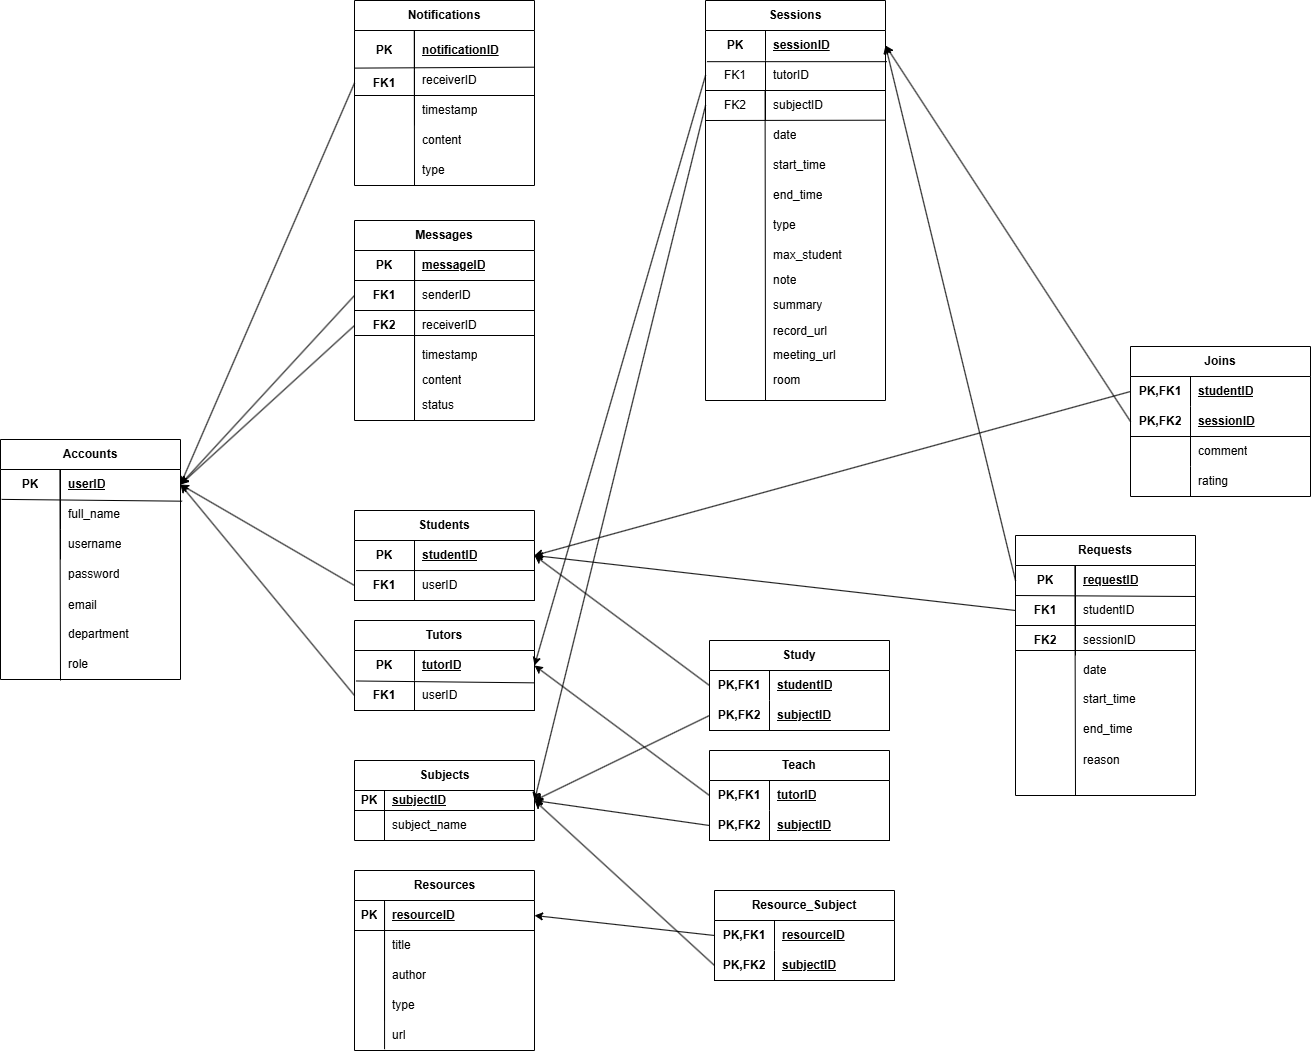
\includegraphics[width=0.8\textwidth]{figures/Kha/mapping.drawio.png}
    \caption{Mapping của hệ thống HCMUT\_Tutor}
\end{figure}

